\documentclass{article}
\usepackage{graphicx} 

\title{Solar System}    
\author{Hayrettin Yazıcı - 150240310} 
\date{November 2025}

\begin{document}    

\maketitle 

\section{Introduction}

Our solar system includes the Sun, eight planets, five officially named dwarf planets, and hundreds of moons, and thousands of asteroids and comets. Our solar system is located in the Milky Way, a barred spiral galaxy with two major arms, and two minor arms. Our Sun is in a small, partial arm of the Milky Way called the Orion Arm, or Orion Spur, between the Sagittarius and Perseus arms. Our solar system orbits the center of the galaxy at about 515,000 mph (828,000 kph). It takes about 230 million years to complete one orbit around the galactic center.

\section{Planets} 

The solar system has eight planets:
\begin{itemize}
    \item Mercury
    \item Venus
    \item \textbf{Earth}
    \item Mars
    \item Jupiter
    \item Saturn
    \item Uranus
    \item Neptune
\end{itemize}



An example drawing of solar system can be seen in the Figure 1.
\ref{fig:solar_system}

\begin{figure}[h]
\centering
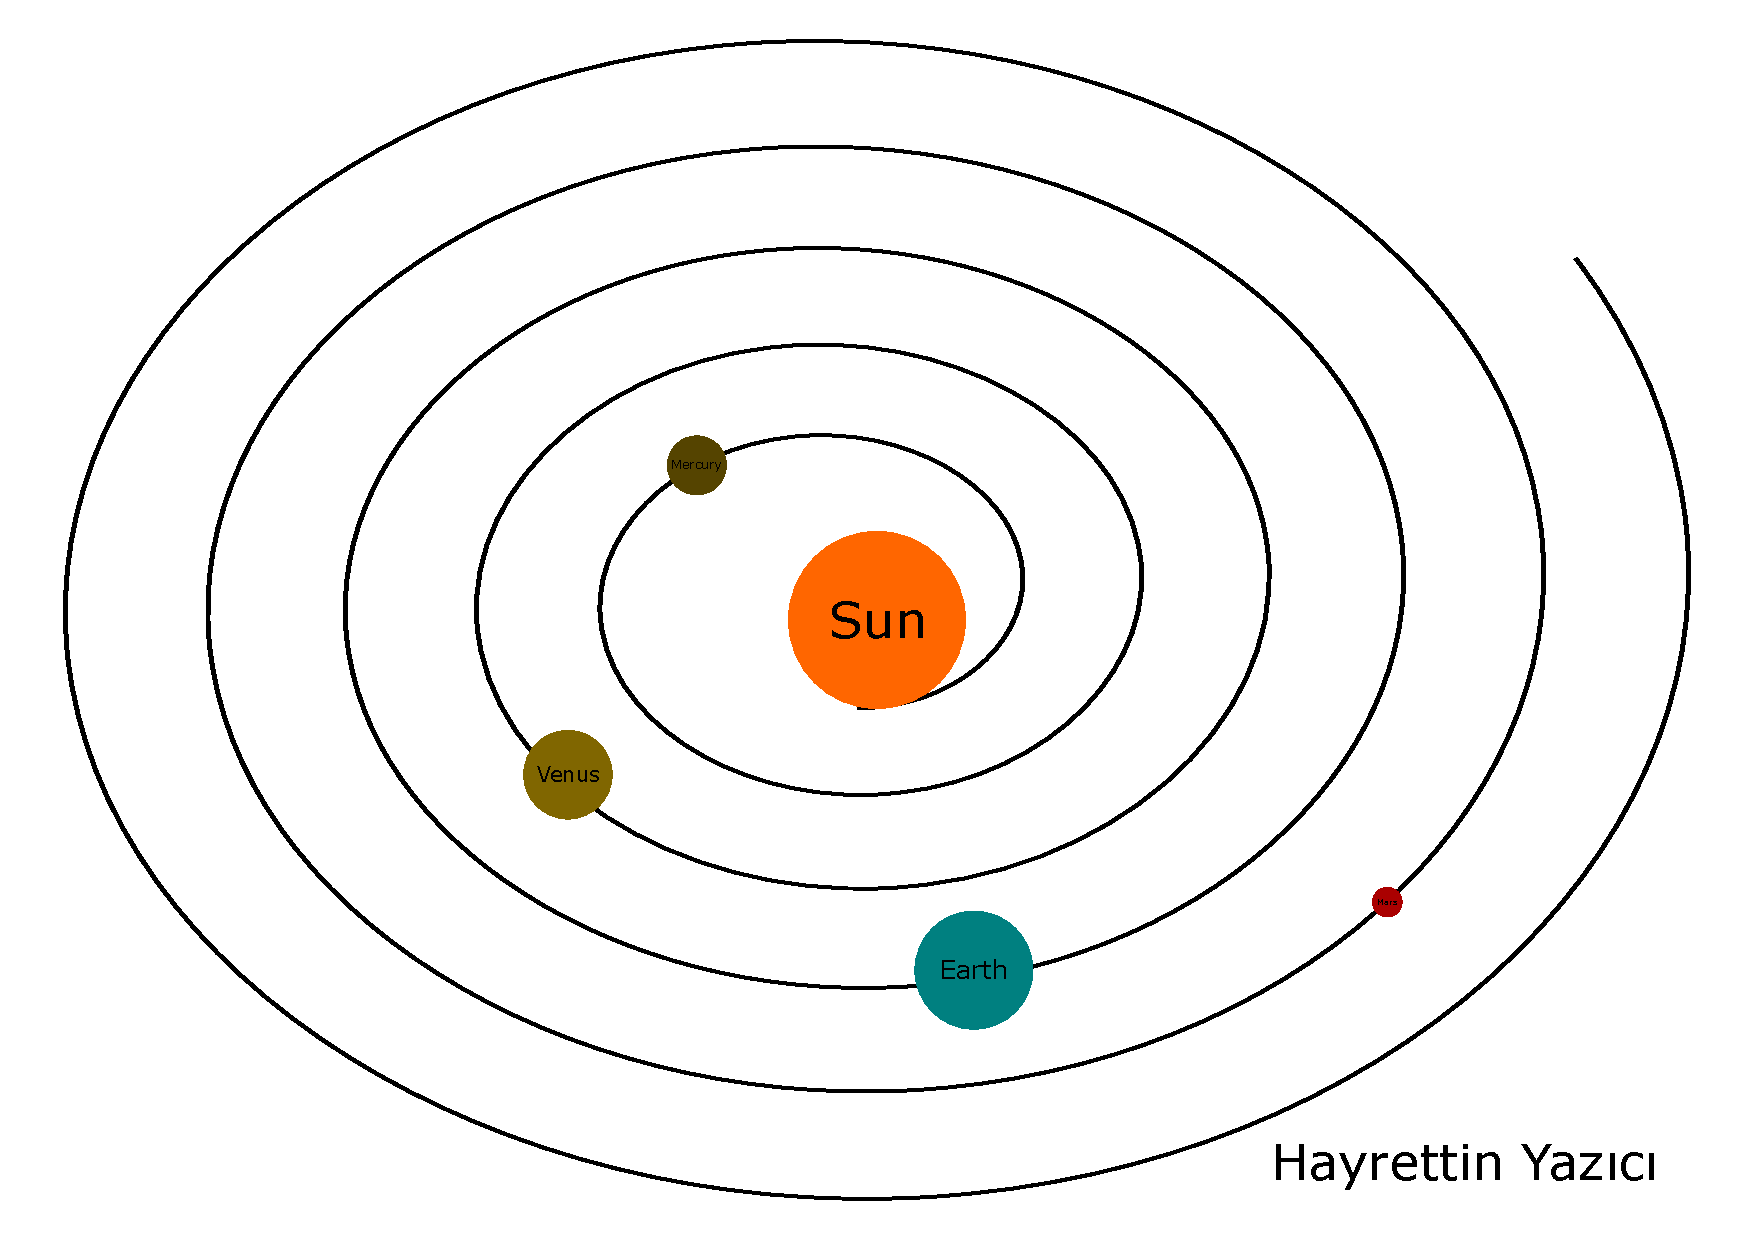
\includegraphics[width=0.5\textwidth]{solar_system.pdf}
\caption{Solar System Drawing}
\label{fig:solar_system}
\end{figure}


\newpage

\subsection{Planet Sizes and Locations}


\begin{table}[h!]
\centering
\begin{tabular}{|c|c|c|}
\hline
\textbf{Planet} & \textbf{Equatorial Diameter (km)} & \textbf{Order from the Sun} \\ \hline
Mercury & 4,880 & 1 \\ \hline
Venus & 12,104 & 2 \\ \hline
Earth & 12,756 & 3 \\ \hline
Mars & 6,792 & 4 \\ \hline
Jupiter & 142,984 & 5 \\ \hline
Saturn & 120,536 & 6 \\ \hline
Uranus & 51,118 & 7 \\ \hline
Neptune & 49,528 & 8 \\ \hline
\end{tabular}
\caption{Names, diameters, and orbital positions of planets}
\label{tab:planets}
\end{table}




As shown in Table \ref{tab:planets}, the planets in our solar system vary greatly in size and distance from the Sun. For instance, \textbf{Jupiter}, with a diameter of 142,984 km, is the \textit{largest}, while \textbf{Mercury}, the \textit{smallest} planet, has a diameter of only 4,880 km. These variations highlight the diversity among the planets orbiting our Sun.

\end{document}  
